%==========================================================
% SIBGRAPI 2026 — Presentation (Beamer)
% Cross-Domain Benchmarking of Nuclei Segmentation Foundation Models
% Compile with pdfLaTeX. Figures are read from ./figures/
%==========================================================
\documentclass[10pt,aspectratio=169]{beamer}

\usetheme{Madrid}
\usecolortheme{whale}
\setbeamertemplate{navigation symbols}{}      % hide nav symbols
\setbeamertemplate{caption}[numbered]
\setbeamerfont{footnote}{size=\tiny}

\usepackage[utf8]{inputenc}
\usepackage{graphicx}
\graphicspath{{figures/}{./}}
\usepackage{booktabs}
\usepackage{adjustbox}
\usepackage{amssymb}
\usepackage{xcolor}

\definecolor{good}{rgb}{0.0,0.55,0.0}
\definecolor{bad}{rgb}{0.78,0.0,0.0}
\newcommand{\win}[1]{\textbf{\color{good}#1}}

%---------------------------------------------------------------
\title[Cross-Domain Nuclei Segmentation]{Cross-Domain Benchmarking of Nuclei\\Segmentation Foundation Models in Histopathology}
\author[IMScience / PUC Minas]{Lucca S.\,P.\ Lacerda \and Matheus Fagundes \and \emph{et al.} \\ \and Z.\,K.\,G.\ Patroc\'inio Jr. \and S.\,J.\,F.\ Guimar\~aes}
\institute[]{Laboratory of Image and Multimedia Data Science (IMScience)\\Pontifical Catholic University of Minas Gerais}
\date{SIBGRAPI 2026}

\begin{document}

\begin{frame}[plain]
  \titlepage
\end{frame}

\begin{frame}{Outline}
  \tableofcontents
\end{frame}

%===============================================================
\section{Motivation}
%===============================================================
\begin{frame}{Why nuclei segmentation --- and why the \emph{contour} matters}
  \begin{itemize}
    \item Nuclei segmentation is a key step in digital pathology: nuclear morphology guides tumor grading and diagnosis.
    \item Two diagnostic features depend directly on the \alert{exact contour}:
      \begin{itemize}
        \item \textbf{Membrane irregularity} --- a smoothed/eroded mask hides the shape deviation that signals malignancy.
        \item \textbf{Chromatin pattern} --- pixel intensity $\propto$ local chromatin density; a leaking mask corrupts the distribution read \emph{inside} it.\footnote{Shifat-E-Rabbi \emph{et al.}, \emph{Cytometry A}, 2025.}
      \end{itemize}
    \item Pretrained ``foundation'' segmenters are increasingly used off-the-shelf.
  \end{itemize}
  \vfill
  \centering
  \footnotesize\emph{We evaluate models not only by \textbf{whether} they detect a nucleus, but by \textbf{how well} they recover its boundary.}
\end{frame}

\begin{frame}{The gap in current evaluations}
  \begin{block}{How foundation models are usually benchmarked}
    On a \alert{test split of the same dataset they were trained on} (e.g.\ PanNuke), with a \alert{single family of metrics} (instance detection / Panoptic Quality).
  \end{block}
  \begin{itemize}
    \item Shows in-distribution performance --- \textbf{not} generalization to new stains, tissues, resolutions.
    \item The ``best'' model can depend on whether the application values precision, recall, or boundary fidelity.
  \end{itemize}
  \vfill
  \centering
  \large\textbf{Practitioner's question:} \emph{which model should I use for \underline{my} images?}
\end{frame}

%===============================================================
\section{Setup}
%===============================================================
\begin{frame}{What we do}
  \begin{itemize}
    \item A deliberately \alert{cross-domain} benchmark of \textbf{4 foundation models}:
      \begin{itemize}
        \item \textbf{Cellpose-SAM} --- flow field + SAM backbone (generalist).
        \item \textbf{CellViT-SAM-H} --- ViT encoder + HoVer-Net decoders.
        \item \textbf{PathoSAM} (micro-sam, ViT-L) --- SAM adapted to microscopy.
        \item \textbf{InstanSeg} --- embedding-based instance segmentation.
      \end{itemize}
    \item On \textbf{4 datasets}: 3 H\&E (oral epithelium, NuInsSeg, CryoNuSeg) + 1 IHC cohort.
    \item \textbf{Multi-metric}: pixel-wise F1, boundary F-score, detection-confidence \textbf{threshold sweep}.
    \item A per-model \alert{in/out-of-distribution provenance map} --- ``unseen'' is checked, not assumed.
  \end{itemize}
\end{frame}

\begin{frame}{Datasets}
  \centering
  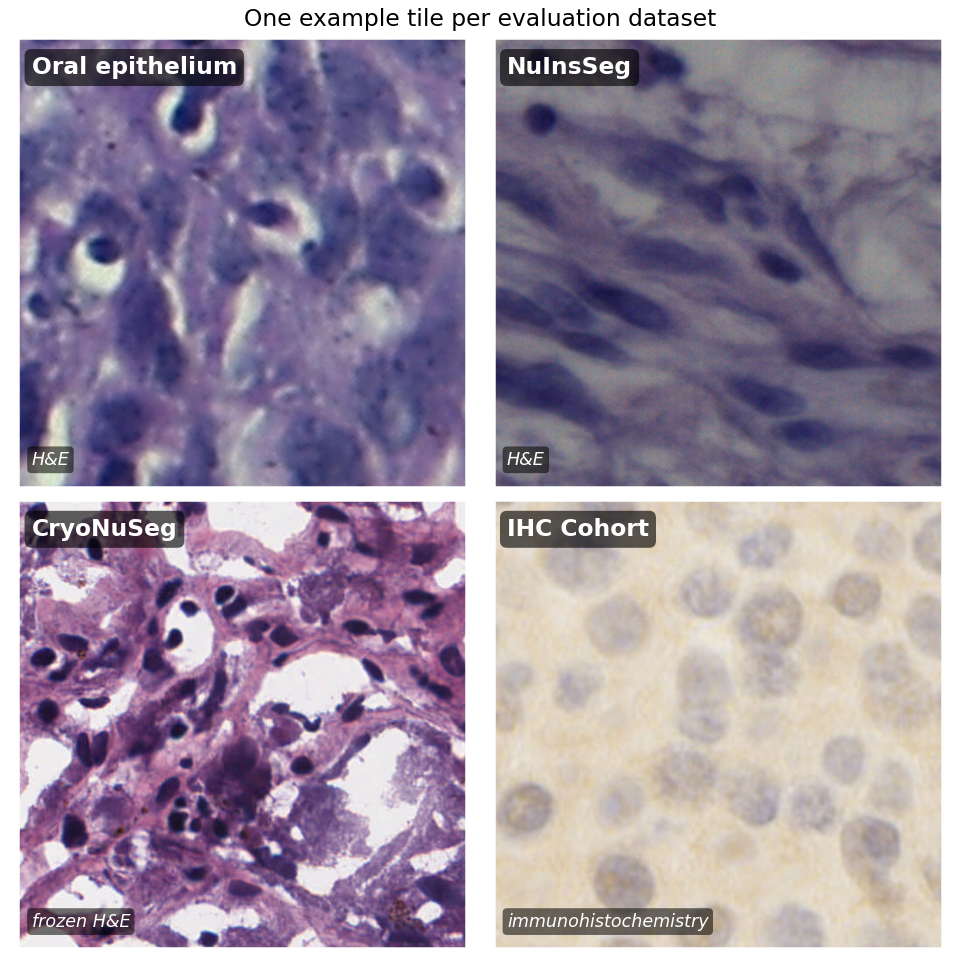
\includegraphics[width=0.62\linewidth]{dataset_examples.png}
  \par\footnotesize
  3 H\&E sets (oral, NuInsSeg, CryoNuSeg) + 1 IHC cohort --- IHC is the hardest cross-modality test (DAB/brown vs.\ H\&E/purple).
\end{frame}

\begin{frame}{Training-data provenance --- honesty up front}
  \centering
  \footnotesize
  \begin{tabular}{lcccc}
    \toprule
    Dataset & Cellpose-SAM & CellViT & PathoSAM & InstanSeg \\
    \midrule
    Oral epithelium & held & held & held & held \\
    NuInsSeg        & \textbf{in} & held & held & \textbf{in} \\
    CryoNuSeg       & \textbf{in} & held & held & held \\
    IHC Cohort      & \textbf{in}$^{*}$ & held & held & \textbf{in}$^{*}$ \\
    \bottomrule
  \end{tabular}
  \vfill
  \begin{itemize}\footnotesize
    \item Transformer models (CellViT, PathoSAM): all four sets are \textbf{held-out}.
    \item Generalists (Cellpose-SAM, InstanSeg): overlap several sets.
    \item \alert{Only oral epithelium is held-out for all four} --- we flag in-distribution cells when reading rankings.
  \end{itemize}
\end{frame}

\begin{frame}{Evaluation protocol}
  \begin{itemize}
    \item Sweep each model's confidence threshold $p \in \{0.1,\dots,0.9\}$ (the precision/recall knob).
    \item \textbf{P --- Foreground pixel-wise F1}: pixel-overlap of the nucleus region.
    \item \textbf{B --- Boundary F-score ($r{=}2$ px tolerance)}: agreement on the \emph{contour} pixels.
    \item Instance F1 (IoU@0.5) and matched-Dice as supporting measures.
  \end{itemize}
  \vfill
  \centering\footnotesize
  Tolerance $r{=}2$ px ($\approx$0.25\% of the diagonal) absorbs $\pm$1--2\,px annotation noise --- stricter than the usual literature default.
\end{frame}

%===============================================================
\section{Results}
%===============================================================
\begin{frame}{Result 1 --- No universal winner}
  \centering
  \scriptsize
  \setlength{\tabcolsep}{4pt}
  \begin{tabular}{l cc cc cc cc}
    \toprule
    & \multicolumn{2}{c}{Oral} & \multicolumn{2}{c}{NuInsSeg} & \multicolumn{2}{c}{CryoNuSeg} & \multicolumn{2}{c}{IHC} \\
    \cmidrule(lr){2-3}\cmidrule(lr){4-5}\cmidrule(lr){6-7}\cmidrule(lr){8-9}
    Model & P & B & P & B & P & B & P & B \\
    \midrule
    Cellpose    & \win{0.811} & \win{0.659} & \win{0.859} & 0.658 & \win{0.845} & \win{0.760} & 0.760 & 0.521 \\
    CellViT-SAM & 0.773 & 0.614 & 0.779 & 0.588 & 0.815 & 0.725 & \win{0.808} & \win{0.535} \\
    PathoSAM    & 0.767 & 0.622 & 0.803 & 0.601 & 0.812 & 0.724 & 0.786 & 0.507 \\
    InstanSeg   & 0.697 & 0.570 & 0.850 & \win{0.664} & 0.784 & 0.696 & 0.747 & 0.500 \\
    \bottomrule
  \end{tabular}
  \vfill
  \begin{itemize}\footnotesize
    \item \textbf{Cellpose} wins all 3 H\&E sets --- \alert{including the held-out oral set} (genuine generalization).
    \item On \textbf{IHC the ranking inverts}: \win{CellViT} leads --- and it never saw that cohort.
    \item[$\Rightarrow$] No single model wins across staining \alert{modalities}.
  \end{itemize}
\end{frame}

\begin{frame}{Result 1 --- the inversion, visually}
  \centering
  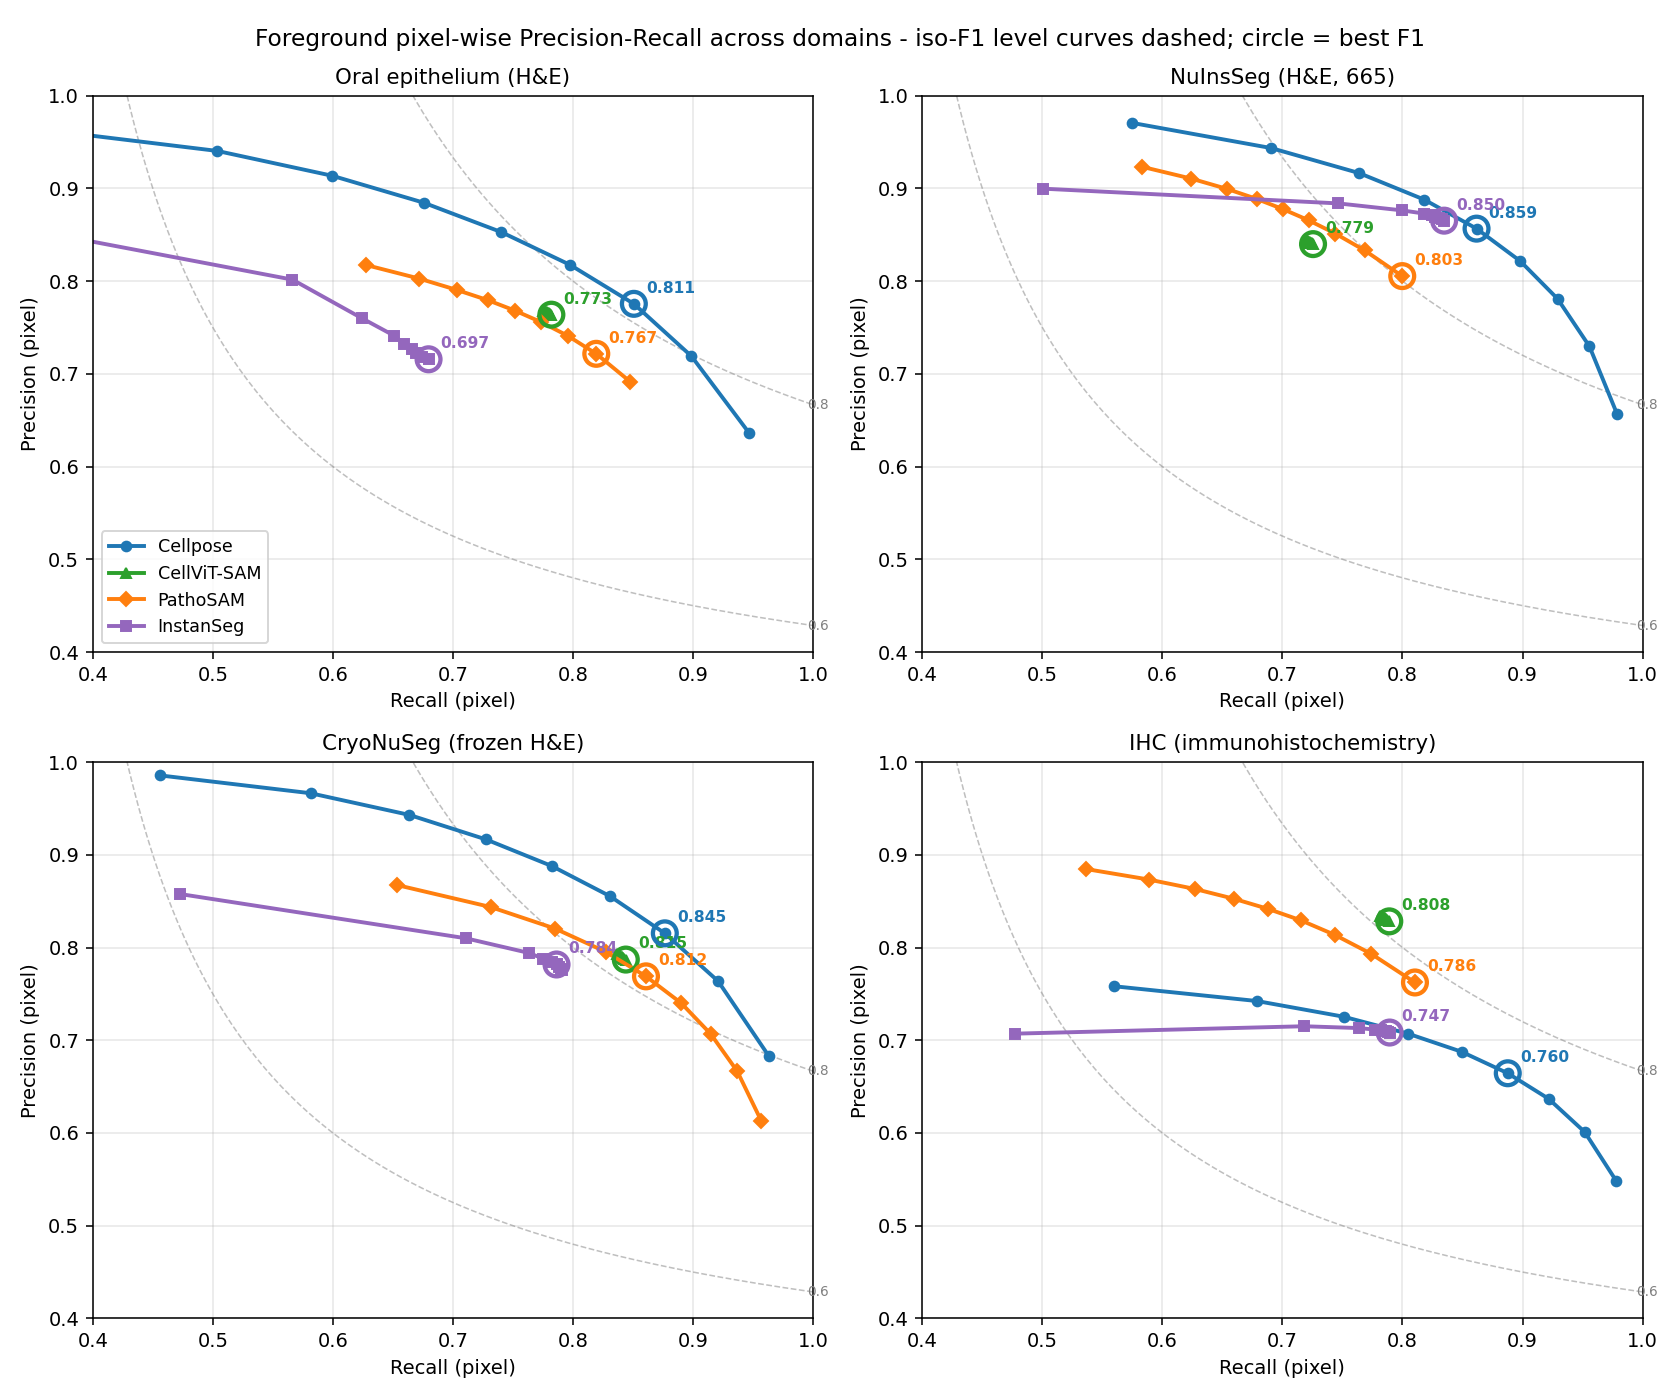
\includegraphics[width=0.82\linewidth]{pr_pixel_crossdomain.png}
  \par\footnotesize
  Pixel-wise PR across domains. Cellpose leads on the 3 H\&E sets; CellViT leads on IHC. Same models, same protocol --- the winner flips with the stain.
\end{frame}

\begin{frame}{Result 2 --- Apparent superiority is a \emph{protocol} effect}
  \begin{columns}
    \begin{column}{0.5\textwidth}
      \begin{itemize}\small
        \item Once a nucleus is \textbf{matched}, all four models trace nearly the same contour: IoU $\approx$0.74--0.76, \textbf{Dice $\approx$0.85}.
        \item The ranking is decided by \alert{how many objects} a model reports, not contour quality.
        \item Over-detectors (CellViT, PathoSAM) accumulate false positives $\rightarrow$ lower precision-weighted scores.
      \end{itemize}
    \end{column}
    \begin{column}{0.5\textwidth}
      \centering
      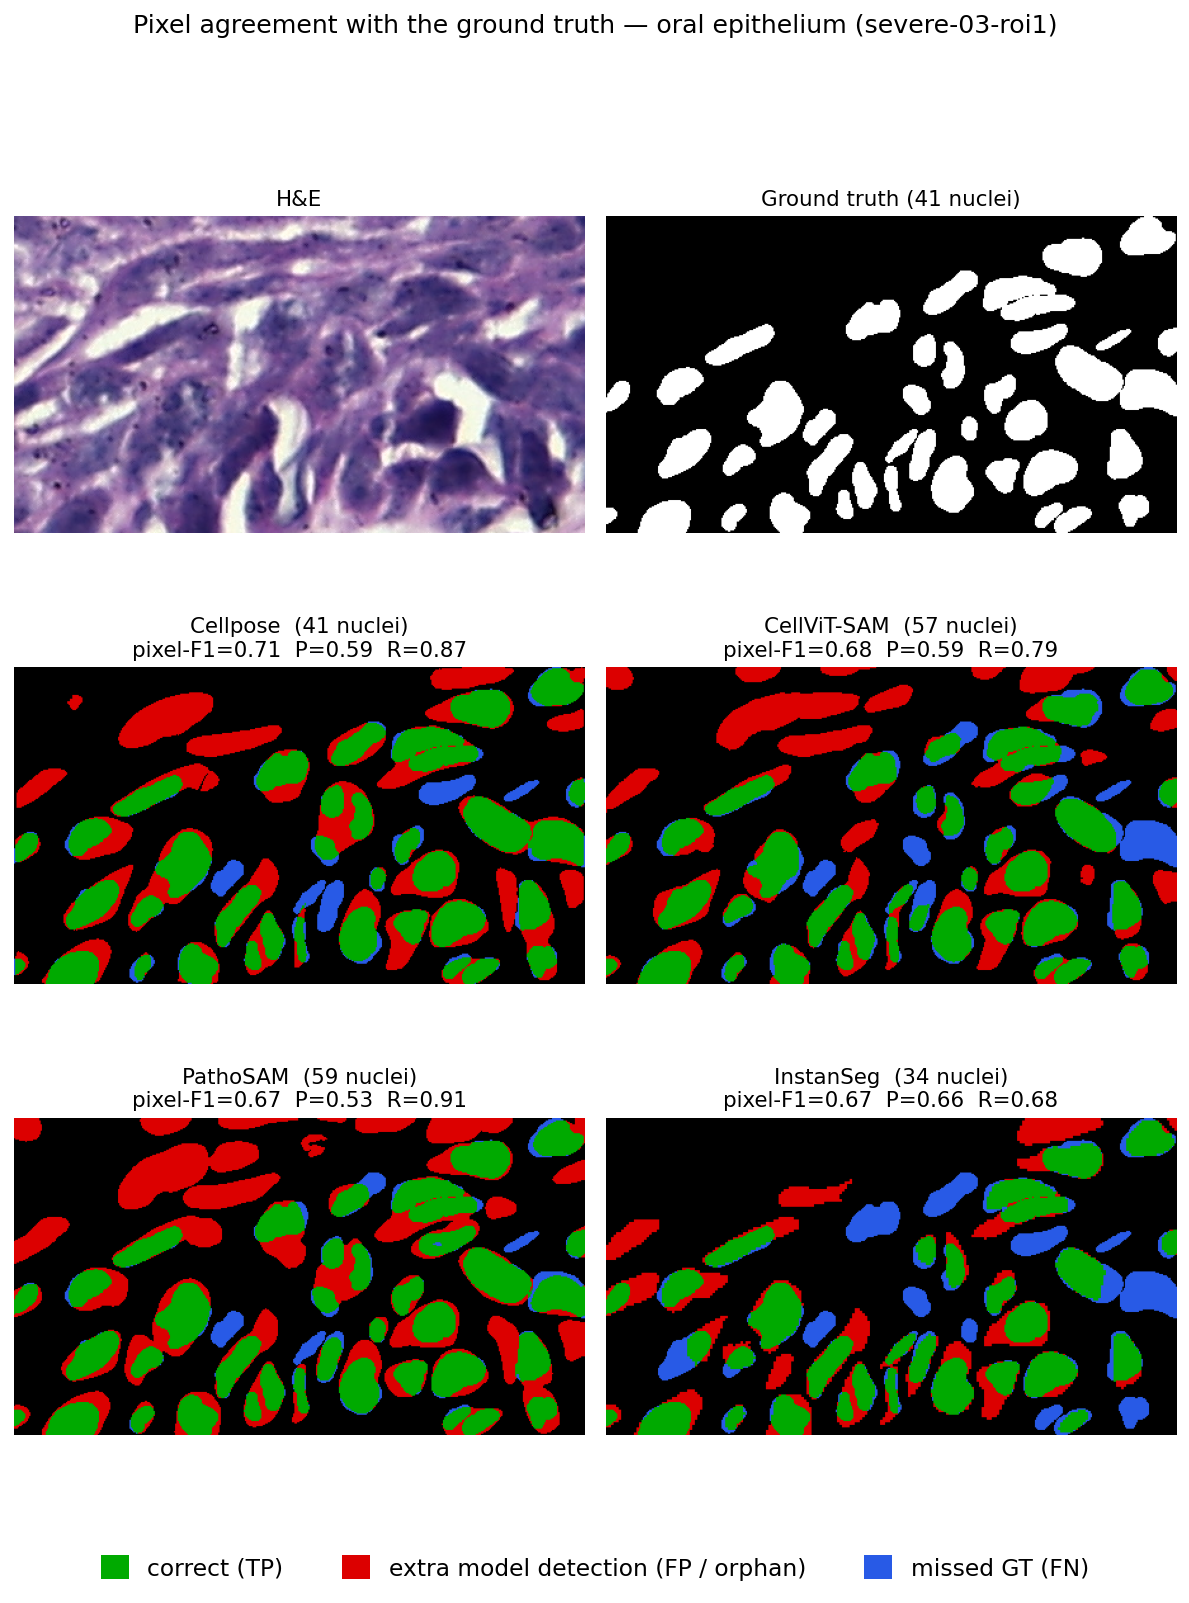
\includegraphics[width=\linewidth]{overlay_oral_protocol.png}
      \par\tiny TP / FP / FN on one oral ROI.
    \end{column}
  \end{columns}
  \vfill
  \footnotesize\alert{Threshold = a tuning knob.} Raise $p$ to suppress FP, lower it to recover missed nuclei --- \emph{except} CellViT, whose saturated probability map leaves it untunable.
\end{frame}

\begin{frame}{Result 3 --- Delineation is \emph{not} solved}
  \begin{itemize}
    \item Dice $\sim$0.85 looks great --- but it is dominated by the \alert{trivial nuclear interior}.
    \item The \textbf{boundary} (B) is recovered far less well: \textbf{B = 0.50--0.76 vs.\ Dice $\sim$0.85}.
    \item B $<$ P in \alert{every} model and \alert{every} domain (gap 0.08--0.28).
  \end{itemize}
  \vfill
  \begin{block}{Why it matters}
    Downstream morphometry reads the chromatin distribution \emph{inside} the mask; an inaccurate boundary perturbs exactly the signal separating benign from malignant nuclei.
  \end{block}
  \centering\footnotesize The contour --- not the interior --- is the part that still needs work.
\end{frame}

\begin{frame}{Result 4 --- Seeded segmentation: the bottleneck is \emph{detection}}
  \centering
  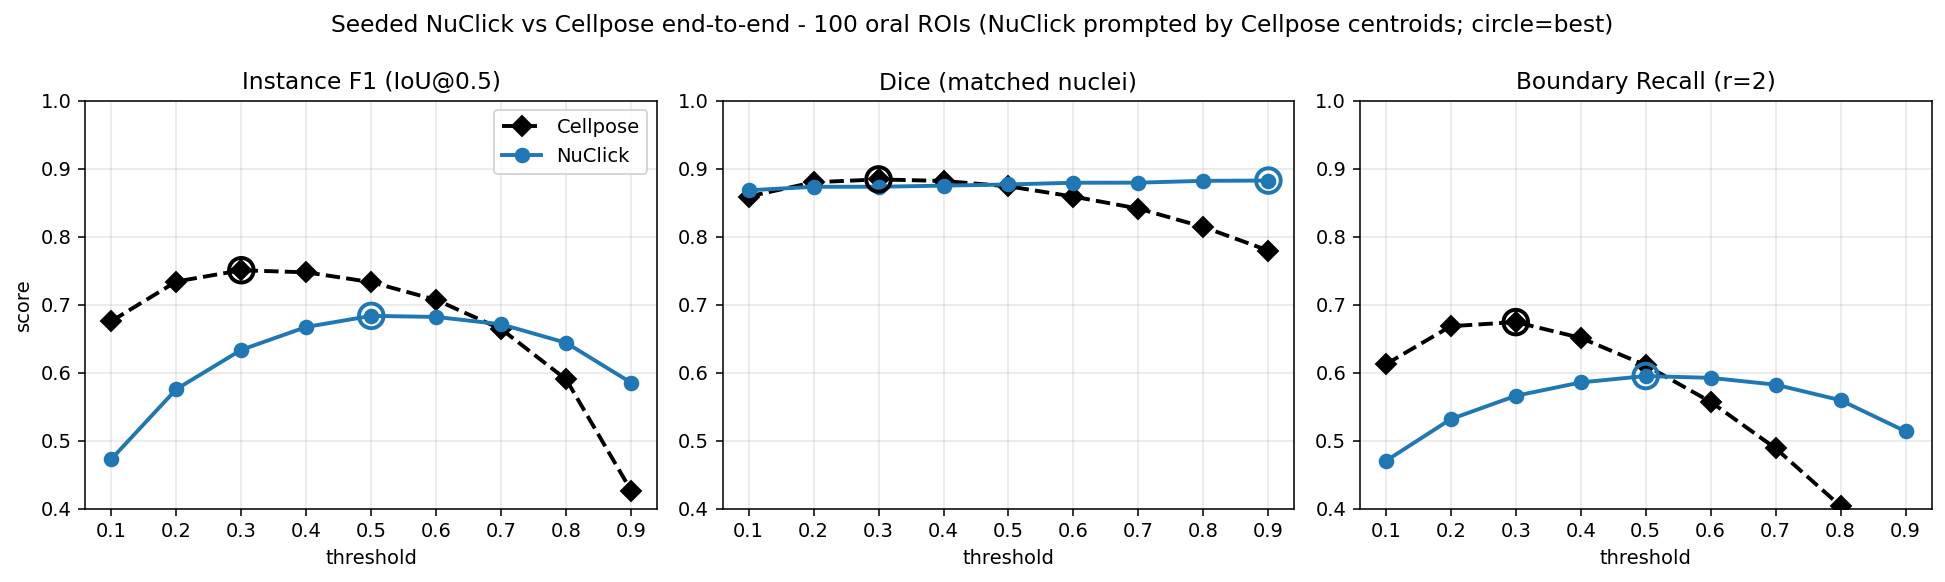
\includegraphics[width=0.92\linewidth]{study_3metrics_full.png}
  \par\footnotesize
  Cellpose\,+\,NuClick (seeded) does \textbf{not} beat end-to-end Cellpose. Across 4 domains a paired bootstrap finds no systematic disadvantage; the gap is which \alert{seeds} it receives --- i.e.\ detection, not delineation.
\end{frame}

%===============================================================
\section{Conclusion}
%===============================================================
\begin{frame}{Conclusion}
  \begin{enumerate}
    \item \textbf{No universal winner} --- the best model flips with the staining modality (Cellpose on H\&E, CellViT on IHC); apparent gaps are often a \emph{protocol} artifact (detection count), not contour quality.
    \item \textbf{Delineation is not solved} --- pixel overlap hides that the diagnostically critical boundary is recovered poorly (B $\ll$ Dice).
    \item \textbf{The remaining gap is detection} --- weak, low-contrast nuclei the models miss entirely; post-hoc segmentation cannot recover them.
  \end{enumerate}
  \vfill
  \begin{block}{Two open problems}
    Recover missed nuclei \emph{without} inflating false positives; recover the exact boundary that carries the morphometric signal.
  \end{block}
  \footnotesize\textbf{Recommendation:} match model + metric to the application; report boundary fidelity alongside overlap.
\end{frame}

\begin{frame}[plain]
  \centering
  \vfill
  {\Large Thank you!}\\[1em]
  {\large Questions?}\\[2em]
  \footnotesize Cross-Domain Benchmarking of Nuclei Segmentation Foundation Models in Histopathology\\
  SIBGRAPI 2026
  \vfill
\end{frame}

\end{document}
